% !TeX program = pdflatex
% =============================================================
% Public Economics -- Lecture 5
% Budget Analysis and Deficit Financing
% Based on: Gruber, J. "Public Finance and Public Policy", Ch. 4
%           (4.1-4.5, Budget Analysis and Deficit Financing)
% Austrian institutional and empirical context added for WU Vienna.
% =============================================================
\documentclass[11pt,aspectratio=169]{beamer}

\usetheme{metropolis}
\usepackage[utf8]{inputenc}
\usepackage[T1]{fontenc}
\usepackage{lmodern}
\usepackage{booktabs}
\usepackage{array}
\usepackage{textcomp}
\usepackage{siunitx}
\usepackage{tikz}
\usepackage{pgfplots}
\pgfplotsset{compat=1.18}
\usepackage{pgf-pie}
\usetikzlibrary{positioning,arrows.meta,calc}

% ----------------------------------------------------------------
% Colors: WU Vienna blue as primary accent
% ----------------------------------------------------------------
\definecolor{wublue}{HTML}{003D7C}
\definecolor{wulight}{HTML}{4F8FC4}
\definecolor{wugray}{HTML}{5C6670}
\definecolor{wured}{HTML}{B0202E}
\definecolor{wugreen}{HTML}{4C8C6B}
\definecolor{wuyellow}{HTML}{D9A441}
\setbeamercolor{palette primary}{bg=wublue,fg=white}
\setbeamercolor{frametitle}{bg=wublue,fg=white}
\setbeamercolor{progress bar}{fg=wublue,bg=wulight!30}
\setbeamercolor{alerted text}{fg=wured}

\setbeamertemplate{frame footer}{Budgeting \& Deficits}
\setbeamertemplate{footline}[frame number]

\title{Public Economics}
\subtitle{Lecture 5 \(\cdot\) Budget Analysis and Deficit Financing}
\author{Shushanik Margaryan}
\institute{WU Vienna University of Economics and Business}
\date{Winter Term}

% Source note command for footnote-style citations on data slides
\newcommand{\srcnote}[1]{{\footnotesize\color{wugray}Source: #1}}

\begin{document}

% =============================================================
\begin{frame}
  \titlepage
\end{frame}

\begin{frame}{Today's Questions}
  \begin{itemize}
    \item Who actually decides what a government spends and taxes each year --- and what stops that process from running an unlimited deficit?
    \item What does it even mean to ``measure'' a deficit correctly --- nominal or real, cash or accrual, actual or cyclically adjusted?
    \item Do today's debts and deficits matter for the long run, and if so, why should we care?
  \end{itemize}
  \vspace{1em}
  \begin{block}{Based on}
    Gruber, J. \emph{Public Finance and Public Policy}, Ch.\ 4 (\S4.1--4.5, Budget Analysis and Deficit Financing).
  \end{block}
\end{frame}

% =============================================================
\begin{frame}{Outline}
  \tableofcontents
\end{frame}

% =============================================================
\section{5.1 The Budget Process}

\begin{frame}{Budgets, Deficits, and Debt: The Basics}
  \begin{block}{Three related concepts}
    \end{block}
    \begin{itemize}
    \item    \textbf{Budget} = planned spending and revenue for a fiscal year.\\
    \item 	\textbf{Deficit} = spending $>$ revenue in a given year (a \emph{flow}).\\
    \item 	\textbf{Debt} = accumulated past deficits (a \emph{stock}).
\end{itemize}


  \vspace{0.3em}
  \begin{itemize}
    \item The EU's \textbf{Maastricht rules} cap the deficit at 3\% of GDP and gross debt at 60\% of GDP for member states  
    \item Every question in this lecture is really about \emph{how} we measure these numbers, and \emph{why} the numbers matter beyond the headline percentage.
  \end{itemize}
\end{frame}

\begin{frame}{Austria's Budget Cycle}
 
  \begin{enumerate}
    \setlength{\itemsep}{3pt}
    \item The \textbf{Bundesministerium für Finanzen (BMF)} drafts the annual budget law (\emph{Bundesfinanzgesetz}, BFG) and the medium-term expenditure framework (\emph{Bundesfinanzrahmengesetz}, BFRG).
    \item The Finance Minister opens the process with the \textbf{Budgetrede} --- the budget speech --- in the Nationalrat, followed by a first reading.
    \item The \textbf{Budgetausschuss} (budget committee) reviews both drafts in detail, supported by the \textbf{Budgetdienst} --- Parliament's own independent budget office.
    \item A structured, multi-day plenary debate follows: general debate, then a chapter-by-chapter (\emph{Untergliederung}) detail debate, then the final vote --- by \textbf{simple majority}; the Bundesrat has no blocking role.
    \item After the fiscal year ends, the \textbf{Rechnungshof} (Court of Audit) prepares the final accounts (\emph{Bundesrechnungsabschluss}) for Nationalrat approval.
  \end{enumerate}
  
\end{frame}

 

\begin{frame}{Der Fiskalrat: Austria's Fiscal Watchdog}
  
  \begin{itemize}
    \item Austria's independent fiscal council traces back to the \textbf{Staatsschuldenausschuss} (1970); it was renamed and reconstituted as the \textbf{Fiskalrat} in \textbf{November 2013}.
    \item Institutionally housed at the \textbf{Oesterreichische Nationalbank (OeNB)} since 1997 
    \item It is Austria's designated \textbf{Independent Fiscal Institution} under EU Regulation: it monitors compliance with national and EU fiscal rules and publishes an annual macro-fiscal outlook.
  \end{itemize}
 
\end{frame}

\begin{frame}{Keeping Bund, Länder, and Gemeinden in Line}
  \small
  \begin{itemize}
    \item Austria is a federal state: the Maastricht deficit and debt ceilings apply to \emph{general} government --- federal, state (\emph{Länder}), and local (\emph{Gemeinden})  combined.
    \item The \textbf{Österreichischer Stabilitätspakt (ÖStP 2012)}, in force since January 2012, is the domestic mechanism that allocates deficit and debt targets --- and sanctions for missing them --- across these three levels.
   \item  Unlike Germany's constitutionally entrenched \emph{Schuldenbremse}, attempts to anchor one in Austria's federal constitution failed to reach the required two-thirds majority --- first in \textbf{December 2011}, then again in the Bundesrat in \textbf{October 2019}. 
   \item Austria's debt brake exists only as \emph{ordinary law}  
   \item The EU Council opened an \textbf{excessive deficit procedure} against Austria on 8 July 2025, triggered by a 2024 deficit of 4.7\% of GDP --- with an approved path requiring the deficit below 3\% by 2028.
  \end{itemize}
 
\end{frame}

 

\begin{frame}{Application: What Happens When a Fiscal Rule Is Relaxed?}
  \small
  \textbf{Grembi, Nannicini \& Troiano (2016)} study a natural experiment in fiscal-rule design: Italy's 1999 national rule restricted municipal deficit growth, but was \textbf{relaxed in 2001} for municipalities under 5{,}000 residents.
  \vspace{0.4em}
  \begin{itemize}
    \item Comparing municipalities just above and below the 5{,}000-resident cutoff, the study finds that once freed from the restraint, municipalities let \textbf{taxes fall} and \textbf{deficits rise}.
    \item The effect was \textbf{larger} where the mayor could be re-elected, where more parties competed, and where voters were older --- consistent with a political-economy story, not just a mechanical budget-constraint effect.
  \end{itemize}
 

  
  \srcnote{Grembi, Nannicini \& Troiano, ``Do Fiscal Rules Matter?'' \emph{AEJ: Applied Economics} 8(3), 2016.}
\end{frame}

% =============================================================
\section{5.2 Measuring the Budget's True Position}

\begin{frame}{Real vs.\ Nominal: The Inflation Tax}
  \small
  \begin{itemize}
    \item Inflation erodes the \emph{real} value of outstanding government debt --- effectively an ``inflation tax'' on whoever holds that debt.
    \item Approximation: $\text{inflation tax (\% of GDP)} \approx \text{debt-to-GDP ratio} \times \text{inflation rate}$.
  \end{itemize}
  \vspace{0.3em}
  \begin{center}
  \begin{tabular}{@{}lc@{}}
    \toprule
    Austria, end-2024 debt-to-GDP & 79.9\% \\
    Austria, average 2024 inflation (HICP) & 2.9\% \\
    \midrule
    Implied inflation tax & $\approx$ 2.3\% of GDP \\
    \bottomrule
  \end{tabular}
  \end{center}
  \vspace{0.3em}

  A deficit measured in purely nominal terms overstates how much the government's real debt burden actually grew.\\
 
\end{frame}

\begin{frame}{Cyclical vs.\ Structural Deficits}
  \small
  \begin{itemize}
    \item Deficits move \textbf{automatically} with the business cycle: recessions cut tax revenue and raise unemployment-related spending, even with no policy change (``automatic stabilizers'').
    \item To judge whether fiscal \emph{policy} is loose or tight, economists strip out the cyclical component to get the \textbf{structural (cyclically adjusted) balance}.
\end{itemize}
\end{frame}

\begin{frame}{Cash vs.\ Accrual Accounting: The International Experience}
 
  \begin{itemize}
    \item \textbf{Cash accounting}: counts revenue/spending when money actually moves. Simple, but treats a euro spent on a durable investment (a bridge) the same as a euro spent on a one-off transfer.
    \item \textbf{Accrual (capital) accounting}: spreads the cost of long-lived investments over their useful life, like a firm's balance sheet --- but is harder to implement and easier to manipulate through valuation assumptions.
  \end{itemize}
  \vspace{0.3em}
  \textbf{International experience is mixed}: \textbf{New Zealand} was the first country to fully implement accrual/capital budgeting (1989) and still uses it; \textbf{Denmark, Finland, and the Netherlands} adopted and later discontinued elements of it; \textbf{Britain} implemented it in 2001 and used it for its 2013 ``Investing in Britain's Future'' plan.
 
\end{frame}

\begin{frame}{Austria's Own Shift: The Haushaltsrechtsreform}
 
  Austria itself moved toward accrual-style budgeting at the federal level, in two stages:
  \begin{itemize}
    \item \textbf{Stage 1 (2009)}: introduced the multi-year BFRG framework and enabled genuine two-year budgets.
    \item \textbf{Stage 2 (2013)}: a wholly new Bundeshaushaltsgesetz (BHG 2013) --- full \emph{Wirkungsorientierte Haushaltsführung} (outcome-oriented budgeting, including mandatory gender budgeting), replacing pure cash accounting (\emph{Kameralistik}) with \textbf{accrual double-entry bookkeeping} across three linked statements:
  \end{itemize}
  \vspace{0.2em}
  \begin{center}
  \begin{tabular}{@{}ll@{}}
    \toprule
    \textbf{Statement} & \textbf{What it tracks} \\
    \midrule
    Ergebnishaushalt & Operating result (like a P\&L) \\
    Finanzierungshaushalt & Cash flow (the traditional cash position) \\
    Vermögensrechnung & Balance sheet of assets and liabilities \\
    \bottomrule
  \end{tabular}
  \end{center}
 
\end{frame}

\begin{frame}{Static vs.\ Dynamic Scoring}
   
  \begin{itemize}
    \item \textbf{Static scoring}: estimates a policy's budget effect holding the size of the economy fixed.
    \item \textbf{Dynamic scoring}: lets the estimate account for how the policy itself changes growth, employment, or behavior --- and therefore future tax revenue.
    \item Dynamic estimates are usually \emph{smaller} in absolute size than static ones for a tax cut, since some of the revenue loss is offset by higher growth --- but they rest on more assumptions, and are correspondingly more contested.
  \end{itemize}
 
\end{frame}

% =============================================================
\section{5.3 Do Debts and Deficits Matter? A Long-Run View}

\begin{frame}{The Tool: Present Discounted Value}
  \begin{block}{Present discounted value (PDV)}
    A euro received (or saved) $t$ years from now is worth less than a euro today. To compare payments across time, discount each future flow by the interest rate $r$:
    \[
      PDV = \frac{F_1}{(1+r)} + \frac{F_2}{(1+r)^2} + \cdots + \frac{F_T}{(1+r)^T}
    \]
  \end{block}
  \vspace{0.3em}
  Any government decision that trades an upfront cost for a stream of future costs or savings --- building infrastructure, cutting taxes today and raising them later, borrowing now to invest --- has to be evaluated this way, \textbf{not} by comparing raw undiscounted totals.
\end{frame}

\begin{frame}{Worked Example: Should the Government Pave the Road?}

  A government can pave a highway with a new ``wear-proof'' material. Paving costs \texteuro{}4 billion \emph{today}, but saves \texteuro{}400 million in maintenance costs at the end of \emph{each} of the next 10 years.
  \vspace{0.3em}
  \[
    PDV(\text{savings}) = \sum_{t=1}^{10} \frac{\text{\texteuro}0.4\text{bn}}{(1+r)^t}
  \]
  \begin{center}
  \begin{tabular}{@{}lccc@{}}
    \toprule
    Discount rate $r$ & 0\% & 4\% & 8\% \\
    \midrule
    PDV of savings & \texteuro{}4.00bn & \texteuro{}3.24bn & \texteuro{}2.68bn \\
    Worth it (cost = \texteuro{}4bn)? & break-even & \textbf{No} & \textbf{No} \\
    \bottomrule
  \end{tabular}
  \end{center}
  
\end{frame}

\begin{frame}{Why Current Debt Labels Can Mislead}
  
  \begin{itemize}
    \item Governments make huge \textbf{implicit} promises --- future pension and healthcare benefits --- that never appear in the officially reported ``debt'' figure, which counts only explicit borrowing.
    \item Relabeling a payment (e.g.\ calling a benefit cut a ``tax increase,'' or vice versa) can leave the government's \emph{true} long-run fiscal position completely unchanged, even though the headline deficit number moves.
  \end{itemize}
  \vspace{0.3em}
 
  This is why economists supplement the official, cash-based debt figure with a much broader concept: the \textbf{present value of all future obligations}, explicit and implicit alike.\\
 
\end{frame}

\begin{frame}{Measuring Long-Run Sustainability: Austria's Pension System}

  The European Commission's \textbf{2024 Ageing Report} projects Austria's public pension expenditure from 2022 to 2070:
  \begin{center}
  \begin{tabular}{@{}lccc@{}}
    \toprule
     & \textbf{2022} & \textbf{Peak (\(\approx\)2032)} & \textbf{2070} \\
    \midrule
    Old-age \& early pensions (\% GDP) & 11.4\% & 12.9\% & --- \\
    Total public pension spending (\% GDP) & 13.7\% & --- & 14.0\% \\
    \bottomrule
  \end{tabular}
  \end{center}
  \vspace{0.3em}
  \begin{itemize}
    \item Spending rises as the baby-boomer generation retires (peaking around 2032), then eases back down --- a net increase of only \textbf{$\sim$0.3 percentage points of GDP} over the full 48-year horizon.
    \item Domestically, the \textbf{Alterssicherungskommission} produces an annual 5-year assessment (due by 30 November) and a long-term report every three years, currently projecting to 2050.
  \end{itemize}

\end{frame}


\begin{frame}{How Far Ahead Should We Look? Budget Windows}
  \small
  \begin{itemize}
    \item A short budget window (one year) misses obligations that only bite later; a very long one (75 years, as US long-run scores sometimes use) is dominated by uncertain assumptions about growth, interest rates, and demographics.
    \item Austria has a rolling \textbf{4-year} window (\S5.1) --- extendable to \textbf{7 years} under the EU's reformed fiscal framework if reforms and investments are committed to.
    \item   There is no ``correct'' window --- only a trade-off between capturing genuinely long-run obligations and trusting projections far enough out that the numbers stop being credible.
  \end{itemize}
 

  
\end{frame}

% =============================================================
\section{Deficits, Crowding Out, and Growth}

\begin{frame}{How a Deficit Can Crowd Out Private Investment}
  \begin{columns}[T]
    \begin{column}{0.55\textwidth}
      \begin{center}
      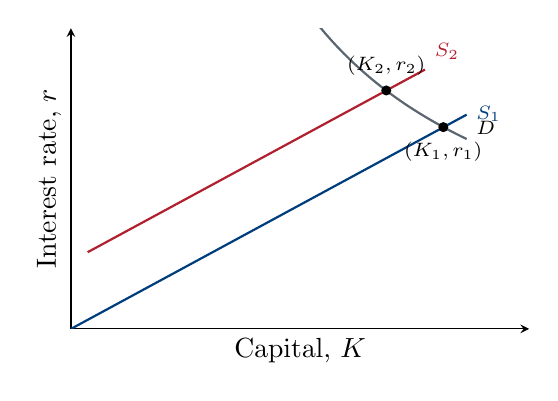
\begin{tikzpicture}
        \begin{axis}[
          width=7.4cm, height=5.4cm,
          xmin=0, xmax=11, ymin=0, ymax=10,
          xlabel={Capital, $K$}, ylabel={Interest rate, $r$},
          axis lines=left,
          ticks=none,
          ]
          \addplot[wugray, thick, domain=1.2:9.5, samples=60] {60/x};
          \node[anchor=west, font=\scriptsize, yshift=4pt] at (axis cs:9.5,6.32) {$D$};
          \addplot[wublue, thick, domain=0:9.5] {0.75*x};
          \node[wublue, anchor=west, font=\scriptsize] at (axis cs:9.5,7.15) {$S_1$};
          \addplot[wured, thick, domain=0.4:8.5] {0.75*(x+3)};
          \node[wured, anchor=south west, font=\scriptsize] at (axis cs:8.5,8.63) {$S_2$};
          \addplot[only marks, mark=*, mark size=1.6pt, black] coordinates {(8.94,6.71) (7.57,7.93)};
          \node[anchor=north, font=\scriptsize] at (axis cs:8.94,6.55) {$(K_1,r_1)$};
          \node[anchor=south, font=\scriptsize] at (axis cs:7.57,8.1) {$(K_2,r_2)$};
        \end{axis}
      \end{tikzpicture}
      \end{center}
    \end{column}
    \begin{column}{0.45\textwidth}
      \footnotesize
      \begin{itemize}
        \setlength{\itemsep}{2pt}
        \item Firms' demand for capital, $D$, meets the supply of private savings --- a deficit means the state borrows from that same pool, which would otherwise fund private investment.
        \item This shifts the supply of loanable funds available to private borrowers left, from $S_1$ to $S_2$.
        \item Equilibrium moves from $(K_1, r_1)$ to $(K_2, r_2)$: interest rates \textbf{rise}, private capital investment \textbf{falls}.
        \item This is the standard \textbf{crowding-out} mechanism.
      \end{itemize}
    \end{column}
  \end{columns}
 
\end{frame}

\begin{frame}{Open Capital Markets Blunt Crowding Out}

  \begin{itemize}
    \item The crowding-out story assumes savings are supplied \emph{domestically} and inelastically. With fully open, integrated international capital markets, a country can borrow from the whole world's savings pool --- so its own deficit barely moves the interest rate it faces.
 	\item As one country inside the euro area's single capital market, Austria effectively faces a supply of savings that is close to perfectly elastic --- far more so than a large economy like the US, where domestic savings still matter enough that some crowding-out concern remains empirically credible.
 \end{itemize}
\end{frame}

\begin{frame}{The Secular Stagnation Puzzle}
  \small
  Real interest rates across the industrialized world have fallen sharply and persistently over the past four decades  \\
  Furman \& Summers (2020) show this decline holds across Canada, France, Germany, Italy, Japan, the UK, and the US alike --- a genuinely worldwide phenomenon, not a US-specific one.\\
  \vspace{0.3em}
  \begin{center}
  \begin{tabular}{@{}lc@{}}
    \toprule
    \textbf{Period} & \textbf{Real interest rate} \\
    \midrule
    Mid-to-late 1980s, average across industrialized nations & $>$5\% \\
    January 2000 (US) & 4.3\% \\
    Pre-Covid, February 2020 (US) & $-$0.1\% \\
    \bottomrule
  \end{tabular}
  \end{center}
  \vspace{0.3em}
  \centering

 
\end{frame}

\begin{frame}{Austria and the Negative-Rate Era}
  \small
  \begin{itemize}
    \item The ECB cut its deposit facility rate below zero in \textbf{June 2014} (to $-$0.10\%), deepening it to $-$0.50\% by \textbf{September 2019} --- and rates stayed negative until \textbf{July 2022}.
    \item Through most of that period, Austrian (and German) long-term government bond yields traded at or below zero: investors were, in effect, \emph{paying} the government to hold their savings.
    \item This an example of  secular-stagnation puzzle 
  \end{itemize}
 
 
  
 
\end{frame}

\begin{frame}{The ``New View'' of Deficits}
 
  \begin{itemize}
    \item If persistently low (or negative) real interest rates mean deficits no longer visibly crowd out private investment, some economists argue fiscal sustainability should be judged by the \textbf{ratio of interest payments to GDP}, not the debt-to-GDP ratio itself.
    \item This does \textbf{not} mean deficits are ``free'': debts must still eventually be serviced, and the argument only strengthens the case for spending that pays for itself --- productive investment with a return above the (low) cost of borrowing.
\end{itemize}
\end{frame}

% =============================================================
 

\begin{frame}[standout]
  Thank you!\\
  \vspace{0.5em}
  \small Questions and discussion
\end{frame}

\end{document}
